\section{PURPOSE AND SCOPE}
The purpose of this calculation is to design the shear connections for 
the \calcproject  project.

\section{GEOMETRY}
Beam shear connections are designed to transfer negligible moments across
joints. The connection may be between beam and beam or between beam and column.
The connection is made using a clip angle that is welded to the connecting beam
and bolted on to the supporting member. This detail is chosen because of the
ease with which it can be fabricated and erected. A typical beam to beam shear
connection is shown in figure \ref{fig:shear_conn}. 

\begin{figure}[h]
    \centering
    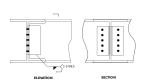
\includegraphics[width=0.5\textwidth]{./images/sc001_1}
    \caption{A shear connection}
    \label{fig:shear_conn}
\end{figure}

\section{MATERIAL SPECIFICATIONS}
The material specifications considered for the design of the shear connections
are as shown in the table \ref{tab:mat_spec}.

\begin{table}[h]
    \centering
    \ttfamily
    \begin{tabular}{ll}
        Element         &Specification\\
        \hline
        Beams           &ASTM A992\\
        Columns         &ASTM A992\\
        Clip angles     &ASTM A36\\
        Bolts           &ASTM F3125\\
        Weld            &FEXX 70\\
        \hline
    \end{tabular}
    \caption{Material specification}
    \label{tab:mat_spec}
\end{table}

\section{DESIGN PHILOSOPHY}
The connection design is done using the open source connection design software Osoconn 
developed by Roshn Noronha, and available at \url{https://osoconn.com}. The connections 
are designed in accordance to the 14th edition AISC 360 specifications using the ASD
method to determine the allowable strength of a connecting element.
The value of the allowable strenght is compared against the required strength, and the ratio 
between the two is calculated as the interaction ratio. If the interaction ratio obtained is 
less that 1.0 then the design is considered satisfactory.
\begin{equation}
    I = \frac{R}{R_a}
\end{equation}
where,

\null\quad\quad \(I\),is the interaction ratio\\
\null\quad\quad \(R\), is the required strength\\
\null\quad\quad \(R_a\), is the allowable strength

The output of the connection design software is provided in Attachment 1.


